\documentclass[preprint,11pt,5p,twocolumn]{elsarticle}
\usepackage{amssymb}
\usepackage{mathtools}
\usepackage{graphicx}
\usepackage{caption}
\usepackage{subcaption}
\usepackage{lineno}

\usepackage[hidelinks]{hyperref}
\usepackage[nameinlink]{cleveref}

\usepackage{afterpage}

\makeatletter
\providecommand{\doi}[1]{%
  \begingroup
    \let\bibinfo\@secondoftwo
    \urlstyle{rm}%
    \href{http://dx.doi.org/#1}{%
      doi:\discretionary{}{}{}%
      \nolinkurl{#1}%
    }%
  \endgroup
}
\makeatother

\begin{document}

\hyphenation{Conv-LSTM}
\hyphenation{Conv-LSTMs}

\begin{frontmatter}

%% Title, authors and addresses

%% use the tnoteref command within \title for footnotes;
%% use the tnotetext command for theassociated footnote;
%% use the fnref command within \author or \address for footnotes;
%% use the fntext command for theassociated footnote;
%% use the corref command within \author for corresponding author footnotes;
%% use the cortext command for theassociated footnote;
%% use the ead command for the email address,
%% and the form \ead[url] for the home page:
%% \title{Title\tnoteref{label1}}
%% \tnotetext[label1]{}
%% \author{Name\corref{cor1}\fnref{label2}}
%% \ead{email address}
%% \ead[url]{home page}
%% \fntext[label2]{}
%% \cortext[cor1]{}
%% \address{Address\fnref{label3}}
%% \fntext[label3]{}

\title{Multi-output Bus Travel Time Prediction\\
Using Convolutional LSTM Neural Network}

\journal{Expert Systems with Applications}

%% use optional labels to link authors explicitly to addresses:
%% \author[label1,label2]{}
%% \address[label1]{}
%% \address[label2]{}

\author{Niklas Christoffer Petersen}

\address{
  Department of Management Engineering \\
  Technical University of Denmark, 2800 Kongens Lyngby \\
  niklch@dtu.dk
}

\begin{abstract}
Accurate and reliable predictions for travel times in a public transport networks is essential for delivering an attractive service.
This paper presents a multi-output, multi-time-step, deep neural network for bus travel time prediction using Convolutional and Long short-term memory (LSTM) layers. The method is evaluated and compared to other popular approaches for link travel time prediction, and currently available services.
\end{abstract}

\begin{keyword}
%% keywords here, in the form: keyword \sep keyword
Bus Travel Time Prediction \sep Intelligent Transport Systems \sep Convolutional Neural Network (CNN) \sep Long short-term memory (LSTM)
\end{keyword}

\end{frontmatter}
\section{Introduction}
Public transport authorities has long found that GPS trajectory data from already deployed \emph{Automatic Vehicle Location}-systems (AVL) can be used in \emph{Intelligent Transport Systems} (ITS) \cite{Tcrp48}. Examples include real-time traffic information for passengers, e.g.\ departure boards, where studies has shown that reliable real-time information at bus stops has a statistical significant dampening effect on the perceived waiting time \cite{Fan2016}.

Besides real-time passenger information, robust arrival- and departure time predictions are necessary for operating more sophisticated ITS applications successfully, e.g.\ demand-adaptive transit systems, and \emph{connection insurance} between different public transport services. Arrival/departure time prediction is commonly approached as a specialization of travel time prediction, where the predicted travel time is simply accumulated downstream the route to yield the arrival/departure time predictions at each stop point of the rest of the current journey. Besides the link travel time, estimations of dwell time (i.e.\ when a bus is holding at a stop point) are also accumulated downstream.

Producing precise bus travel time predictions in areas with little external influence, e.g.\ rural areas, can be solved to a large extent with historical averaging or simple regression methods \cite{Williams2003,Altinkaya2013}. The problem becomes much more complex in urban areas where congestion, events, road-works, weather, etc.\ highly influences the traffic flow and passenger demand.

In this paper we presents a multi-output, multi-time-step deep neural network for bus travel time prediction using a combination of \emph{Convolutional} and \emph{Long short-term memory} (LSTM) \cite{Lstm1,Lstm2} layers. The goal of this work is to produce precise short-term predictions (e.g.\ $0-1.5$ hours) for link travel time, specifically for bus traffic in urban areas. The method is evaluated and compared to other popular approaches for link travel time prediction, and currently available services.

The paper is structured in the following manner: In the next section related work and literature is reviewed. \Cref{sec:convlstm} introduces Convolutional LSTM neural networks in general and in \Cref{sec:model} we present the proposed multi-output model in more details, including e.g.\ network topology, etc. \Cref{sec:experiments} introduces the Copenhagen-dataset, which the model has been evaluated on, and our results are presented and discussed in~\Cref{sec:results}. Finally we conclude on the work in~\Cref{sec:conclusion}.

\subsection{Literature review}
Early approaches presents historical averaging models \cite{Dailey1999,Sun2007}, and linear regression \cite{Patnaik2004}. Recent research presents this type of model only for comparison purpose, and the models are in all cases outperformed by the compared models \cite{Shalaby2004,Jeong2005}. Kalman-filters, which by its capabilities of maintaining state between predictions, has shown interest from several studies, either as an independent model \cite{Chen2001,Shalaby2004} or in combination with other models \cite{Zaki2013,Bai2015}. 

Both the different regression style models and the Kalman-filter models still has limited options for capturing fluctuations in travel and dwell time in a metropolitan bus system, since they to a large extent still is averaging and smoothing their response. E.g., the Kalman-filter's state is only directly accessible for the leading time-step, and thus not capable of finding long-distance patterns spanning over several links and/or over several time-steps. This is substantiated by \cite{Lin2013} and \cite{Kumar2014} that finds artificial neural networks (ANN) outperforms Kalman-filter models.

The computational challenges of pure ANN approaches i.a.\ has sparked the interest for studying composite or hybrid models. \citet{Zaki2013} uses a two-stage approach by combining offline ANN-models, with an adaptable/online Kalman-filter to yield a dynamic model. The model is not actually learning in the long term, but is able to adapt to temporal variations in the current travel time on a journey.

Some recent research recognizes that several routes can benefit from each other's predictions if they share some partial route segment, e.g.\ \cite{Yu2011,Gal2014,Bai2015}, however none of these approaches consider cross temporal correlations between different route segments, and only uses a small window for correlation with upstream links (e.g.\ max. 3 links).

Finally \citet{YanjieDuan2016} proposes to use LSTM model for general highway travel time prediction, and do predict multiple steps ahead, but only for a single link at a time, i.e.\ cross link (spacial) correlations are lost.

\section{Convolutional LSTM neural networks}
\label{sec:convlstm}
A Long short-term memory (LSTM) neural network is a special type of Recurrent Neural Network~(RNN) which has proven robust for capturing long-distance dependencies \cite{Lstm1,Lstm2}. The important feature of a LSTM network is its capability to persist cell state, $c_t$, from previous observations across sequences of input (e.g.\ time), but also eliminate information which is considered unimportant. To allow this mechanism the persistence of information is controlled by three gates: \emph{input gate}, \emph{forget gate}, and \emph{output gate}. Each gate yields a state value at time $t$, respectively $i_t$, $f_t$, and $o_t$, along with the cell output, $h_t$, cf.\ \Cref{eq:lstm}, where $\circ$ denotes the entry-wise product.

\begin{equation}
\begin{aligned}
  i_t &= \sigma \left( W_\mathit{xi} x_t + W_\mathit{hi} h_{t-1} + W_{ci} \circ c_{t-1} + b_i \right) \\
  f_t &= \sigma \left( W_\mathit{xf} x_t + W_\mathit{hf} h_{t-1} + W_\mathit{cf} \circ c_{t-1} + b_f \right) \\
  c_t &= f_t \circ c_{t-1} + i_t \circ \mathrm{tanh} \left( W_\mathit{xc} x_t + W_\mathit{hc} h_{t-1} + b_c \right) \\
  o_t &= \sigma \left( W_\mathit{xo} x_t + W_\mathit{ho} h_{t-1} + W_\mathit{co} \circ c_{t} + b_o \right) \\
  h_t &= o_t \circ \mathrm{tanh} \left( c_t \right)
\end{aligned}
\label{eq:lstm}
\end{equation}
\vspace{.5em}

\Cref{fig:lstm-peepholes} illustrates the inner structure of a LSTM cell with peephole as proposed by \cite{LstmPeephole}. 
Is has especially grown popular for predicting time series using methods evolved from \cite{LstmTs}, where fixed-length windows of time-series are generated and feed into a LSTM network. Multiple LSTMs can be stacked such more complex patterns of sequential information (e.g.\ temporal patterns) can be learned.

\begin{figure}[!ht]
  \centering
  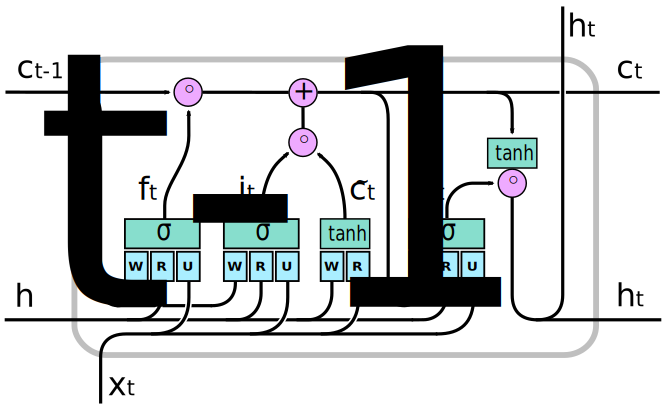
\includegraphics[scale=.45]{drawings/lstm-peepholes.pdf}
  \caption{Structure of LSTM cell with peephole.}
  \label{fig:lstm-peepholes}
\end{figure}

Convolutional Neural Networks~(CNN) on the other hand has been widely used for capturing spacial relationships, e.g.\ importance of neighboring pixels in an image. As opposed to fully connected layers, where each unit, $i$, in the layer, has a dedicated scalar weight, $w_{ij}$, for all input value, $x_j$, convolutional units are only locally connected and reuses the same weights for producing several outputs. Instead of considering the entire input-vector, only a fixed sized window, or \emph{convolution}, around each input is considered. The weights are therefore referred to as the \emph{filters} or \emph{kernels} of the layer. \Cref{fig:conv} illustrates a single convolutional filter of size $3$ being applied to 1-dimensional data.

\begin{figure}[!ht]
  \centering
  \includegraphics[scale=.45]{drawings/conv.pdf}
  \caption{Application of Convolutional filter onto 1D data.}
  \label{fig:conv}
\end{figure}

Special care needs to be taken on the boundaries, i.e.\ where the convolutional filter will exceed the input. A popular approach to avoid the size of the output decreases is to pad the input, e.g.\ with zeros. This ensures that the output shape of each convolutional unit will always be identical to the input shape, which is often desirable. One of the key benefits of convolutional networks is that the number of weights that needs to be learned is considerably reduced compared to fully connected networks, and that learned patterns can be transfered across space. I.e.\ the convolutional filters become feature detectors, that in our case can detect spacial patterns across links, e.g.\ congestion forming, etc.   

\citet{ConvLSTM} introduced the novel combination of Convolutional and LSTM layers into a single structure, the \emph{Convolutional LSTM}, or simply \emph{ConvLSTM}. Specifically the method applies convolutional filters in the \emph{input-to-state} and \emph{state-to-state} transitions the LSTM cf.\ \Cref{eq:convlstm}, where $*$ denotes the convolution operator.

\begin{equation}
\begin{aligned}
  i_t &= \sigma \left( W_\mathit{xi} * x_t + W_\mathit{hi} * h_{t-1} + W_{ci} \circ c_{t-1} + b_i \right) \\
  f_t &= \sigma \left( W_\mathit{xf} * x_t + W_\mathit{hf} * h_{t-1} + W_\mathit{cf} \circ c_{t-1} + b_f \right) \\
  c_t &= f_t \circ c_{t-1} + i_t \circ \mathrm{tanh} \left( W_\mathit{xc} * x_t + W_\mathit{hc} * h_{t-1} + b_c \right) \\
  o_t &= \sigma \left( W_\mathit{xo} * x_t + W_\mathit{ho} * h_{t-1} + W_\mathit{co} \circ c_{t} + b_o \right) \\
  h_t &= o_t \circ \mathrm{tanh} \left( c_t \right)
\end{aligned}
\label{eq:convlstm}
\end{equation}
\vspace{.5em}

The output dimensionality of a \emph{ConvLSTM} layer is like the traditional CNN-layer determined by the number of filters applied. However \emph{ConvLSTM} requires a total of eight filters for each desired output, i.e.\ four \emph{input-to-state} filters ($W_\mathit{xi}$, $W_\mathit{xf}$, $W_\mathit{xc}$, and $W_\mathit{xo}$) and four \emph{state-to-state} filters ($W_\mathit{hi}$, $W_\mathit{hf}$, $W_\mathit{hc}$, and $W_\mathit{ho}$).

% Hmm, i really would like this to get numbered before fig:data_shape, but cant make it work.
\afterpage{
\begin{figure*}[!t]
  \centering
  \includegraphics[scale=.75]{drawings/conv_lstm.pdf}
  \caption{Convolutional LSTM network topology.}
  \label{fig:ConvLSTM}
\end{figure*}
}
%\newpage

\section{Multi-output model}
\label{sec:model}
In this section we present the multi-output, multi-time-step model for bus travel time prediction, which uses the \emph{ConvLSTM} introduced in the previous section.

\subsection{Network topology}


\Cref{fig:ConvLSTM} shows the overall network topology, where blue boxes illustrates \emph{input-to-state} convolutions and yellow \emph{state-to-state} convolutions. The network uses an encoder/decoder technique that to a large extent follows \cite{ConvLSTM}, where the encoder-block consists of two \emph{ConvLSTM} layers. The result is feed into a decoder, or prediction block, also consisting of two \emph{ConvLSTM} layers. The architecture allows unequal $w$ and $k$, e.g.\ predict the next $3$ time-steps based on a window size of $20$.

Thus convolutional filters are applied to each input, at each time-step, to the respective LSTM-cell, and also between LSTM-cells in the state-transition. Since the time-steps are one-dimensional~(i.e.\ link travel times across links), the filters are also one-dimensional. In each of the two blocks, the \emph{ConvLSTMs} are arranged with filter sizes of respectively $10\times1$ and $5\times1$ for each of the layers in the block. This size is used both for the \emph{input-to-state} and \emph{state-to-state} convolutional filters. Finally each \emph{ConvLSTM} layer 64~outputs, yielding a total of 512 convolutional filters.

To avoid over-fitting doing training \emph{Dropout} \cite{Dropout} is performed between the \emph{ConvLSTM} layers, and \emph{Batch Normalization} \cite{BatchNorm} are also performed before each \emph{ConvLSTM} layer to ensure reasonable input for activations. The dropout factor is adjusted to respectively 20\%, 10\% and 10\%.

Each of the \emph{ConvLSTM} layers uses linear activation functions, and the output from the last layer in the decoder-block is feed into a fully connected (FC) layer using the \emph{ReLU} activation function, which also ensures only positive travel times are predicted.

\subsection{Data preparation}
We expect link travel times from AVL-systems to be available in a tabular form, where each link travel time measurement has a timestamp, and a reference to the link as illustrated in~\Cref{tab:data}.
\begin{table}[!ht]
  \centering
  \footnotesize
  \begin{tabular}{llr}
    Timestamp & Linkref. & Link travel time (s) \\ \hline \hline
    2017-10-10 00:20:02 & 29848:1254 & 63 \\ \hline
    2017-10-10 00:21:07 & 1254:1255  & 65 \\ \hline
    2017-10-10 00:21:51 & 1255:10115 & 44 \\ \hline
    \vdots & \vdots & \vdots 
  \end{tabular}
  \caption{Example of raw travel time measurements.}
  \label{tab:data}
\end{table}

For the \emph{ConvLSTM} model to be able to capture the desired spatial-–temporal patterns, the input data must be arranged in a suitable manner: I.e.\ in $N$ samples, each with a window of the $w$ lagging time-steps $t-w+1, \ldots, t$, and each time-step with $u$ link travel times $1, \ldots, u$ cf.~\Cref{fig:data_shape}.

Likewise is the output arranged with $N$ predictions of $k$ time steps ahead, $t+1, \ldots, t+k$. Thus the input is a 4D-tensor with shape $(N, w, u, 1)$, and the output a 4D-tensor with shape $(N, k, u, 1)$ -- in both bases the last one refers to the single link travel time for each time-step/link combination. It is emphasized that each prediction consists of travel time predictions for all links for the next $k$ time-steps, i.e.\ multi-output, multi-time-step prediction.

The $N$ samples are sampled at a fixed time resolution, since we need a shared time reference across all links. \Cref{sec:experiments} elaborates on some of the considerations in choosing a sound resolution.

\begin{figure}[!ht]
  \centering
  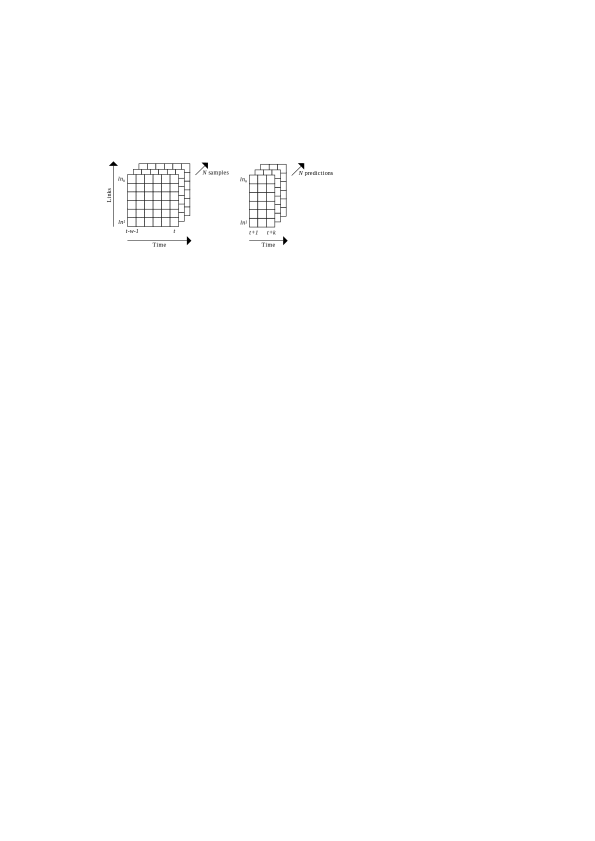
\includegraphics[scale=1.1]{drawings/data_shape.pdf}
  \caption{Shapes of the input and output data.}
  \label{fig:data_shape}
\end{figure}

\subsection{Detrending}
Urban bus travel times varies throughout the time of the day, and the day of the week due to \emph{recurring congestion}. In order to reduce the need for the network to learn this recurring variation, link travel for link $\mathit{ln} \in \{ 1,\ldots,u\}$, at time-step $t$, $x_{\mathit{ln},t}$, is normalized to focus on deviations from the normal and expected pattern. Travel times are centered with the mean for each link, at the time of day, and day of week, $\mathit{\bar{x}_{\mathit{ln},\mathit{dow},\mathit{tod}}}$, and scaled with the standard deviation for each link, $\sigma_\mathit{ln}$, cf.\ \Cref{eq:normalization}.

\begin{equation}
  x'_{\mathit{ln},t} = \frac{x_{\mathit{ln},t} - \bar{x}_{\mathit{ln},\mathit{dow},\mathit{tod}}}{\sigma_\mathit{ln}}
  \label{eq:normalization}
\end{equation}

A similar normalization is applied to the predicted travel times, $y_{\mathit{ln},t}$, but only using the historical mean and standard deviation, since the true mean and standard deviation obviously is unavailable in real-time prediction scenarios.

When calculating the mean and standard deviation it can be beneficial to exclude extreme outliers, since both mean and standard deviation are higly sensitive to such measurements. A suggested method is to apply \emph{absolute deviation around the median} (MAD) cf.~\cite{Olewuezi2011} when calculating $\mathit{\bar{x}_{\mathit{ln},\mathit{dow},\mathit{tod}}}$ and $\sigma_\mathit{ln}$.


\subsection{Training}
The network is trained using the \emph{RMSprop}-algorithm \cite{RMSprop}.

During training the variables $\mathit{\bar{x}_{\mathit{ln},\mathit{dow},\mathit{tod}}}$ and $\sigma_\mathit{ln}$ should be calculated solely based on the training set, to emulated real-world application.

\begin{figure*}[!t]
    \centering
    \begin{subfigure}[t]{0.31\textwidth}
        \centering
        \includegraphics[width=\textwidth]{plots/decycle_5min.pdf}
        \caption{5 min}
    \end{subfigure}%
    ~ 
    \begin{subfigure}[t]{0.31\textwidth}
        \centering
        \includegraphics[width=\textwidth]{plots/decycle_15min.pdf}
        \caption{15 min}
    \end{subfigure}
    ~
    \begin{subfigure}[t]{0.31\textwidth}
        \centering
        \includegraphics[width=\textwidth]{plots/decycle_30min.pdf}
        \caption{30 min}
    \end{subfigure}

    \caption{Examples of travel time for a single link at various time resolutions.}
    \label{fig:resolutions}
\end{figure*}
\newpage

\section{Experiments}
\label{sec:experiments}

For evaluation the method is applied to a dataset from Copenhagen's public transport authority, ``Movia''. The dataset consists of 1,2~M~travel time observations for the ``4A'' bus line in the period January 1 to August 31 2017. The data points were collected using the real-time AVL-system installed in all vehicles of the line. 

\begin{figure}[!ht]
  \centering
  \includegraphics[width=0.4\textwidth]{drawings/map.png}
  \caption{Geography of the 4A bus line in Copenhagen.}
  \label{fig:4a_map}
\end{figure}

The geography of the route is shown in \Cref{fig:4a_map}. As the line circles Central Copenhagen, it is potentially highly sensitive to congestion to/from the city as it intersects with several large corridors along its route. Southeast of the city center the lines splits in different destination patterns (gray), therefore only the first 32 links are considered in this experiment (red).

\subsection{Data preprocessing}
Furthermore, to allow predictions for fixed time-steps ahead, data was aggregated at a fixed resolution. \Cref{fig:resolutions} shows examples of travel time for a single link and a single day at various time resolutions. The red dots are actual measurements, and the blue line the aggregated resolution. The choice depends of the \emph{expected} frequency of the line, and is a balance between capturing the details and still having a reasonal number of measurements in each time-step.

For this expirement data was aggregated into 15-minute time-steps and normalized cf.~\Cref{sec:model}.



The implementation of the proposed model was done in Python using Keras \cite{Keras}.




%TODO: How much used for training, how much for testing?
\subsection{Evaluation}
In order to evaluate the presented model and comparisons, the following measures is used: \emph{mean absolute error} (MAE), \emph{root mean square error} (RMSE), and \emph{mean absolute percentage error} (MAPE) cf.~\Cref{eq:mae,eq:rmse,eq:mape}, where $X_i$ is the true travel time for sample $i$ and $\widehat{X}_i$ is the predicted travel time.

\begin{equation}
    \textrm{MAE}(X, \widehat{X}) = \frac{\sum_{i = 1}^{n} \left| X_i - \widehat{X}_i \right| }{n}
    \label{eq:mae}
\end{equation}

\begin{equation}
    \textrm{RMSE}(X, \widehat{X}) = \sqrt{\frac{\sum_{i = 1}^{n} \left(X_i - \widehat{X}_i \right)^2}{n}}
    \label{eq:rmse}
\end{equation}

\begin{equation}
    \textrm{MAPE}(X, \widehat{X}) = \frac{1}{n} \sum_{i = 1}^{n} \left| \frac{X_i - \widehat{X}_i}{X_i} \right| 
    \label{eq:mape} 
\end{equation}

\section{Results and discussion}
\label{sec:results}
The model is trained on the prepared data using a sliding window approach to simulate real-world conditions where real-time travel time measurements arrives as a continuously data stream. \Cref{fig:loss} shows the evolution of training and validation loss for each epoch for such a window, where the loss is the MAE if the individual links.

\begin{figure*}[!ht]
  \centering
  \includegraphics[width=0.75\textwidth]{plots/comparison_day.pdf}
  \caption{}
  \label{fig:comparison_day}
\end{figure*}

d
\begin{figure}[!ht]
  \centering
  \includegraphics[width=0.4\textwidth]{plots/conv_lstm_model_loss.pdf}
  \caption{Training and validation loss evolution. TODO: Needs to be updated ...}
  \label{fig:loss}
\end{figure}

\Cref{tab:results} shows the results of the presented method and compares to two other methods: 1) a naïve historical average model, i.e. equivalent of just prediction the normalized value, $\bar{x}_{l,\mathit{dow},\mathit{tod}}$ and 2) a pure LSTM model as proposed by \cite{YanjieDuan2016}. Predictions are accumulated downstream on journey level to simulate for use in real-time bus arrival/departure time prediction.

From the table it is found that the Convolutional LSTM performs better than the compared methods. Although the advantage might seem small it is emphasized that evaluation measurements are averaging their response, and thus the increased accuracy can be much higher on individual journeys, especially if they experienced very irregular travel times.

\begin{table*}[!ht]
    \caption{Results of the presented and other popular models}
    \label{tab:results}
    \center
    \begin{tabular}{ll|rrr}
        Model & Time ahead & MAE (min) & RMSE (min) & MAPE (\%) \\
        \hline 
        Historical average &                & 4.90 & 6.32 & 7.38 \% \\ 
        \hline 
        Current Model      & t + 1 (15 min) &  &  &  \% \\ 
        Current Model      & t + 2 (30 min) &  &  &  \% \\ 
        Current Model      & t + 3 (45 min) &  &  &  \% \\ 
        \hline 
        Pure LSTM          & t + 1 (15 min) & 3.71 & 3.71 & 5.87 \% \\
        Pure LSTM          & t + 2 (30 min) & 4.31 & 5.63 & 6.63 \% \\
        Pure LSTM          & t + 3 (45 min) & 4.97 & 6.41 & 7.52 \% \\
        \hline 
        Convolutional LSTM & t + 1 (15 min) & 2.96 & 3.94 & 5.10 \% \\
        Convolutional LSTM & t + 2 (30 min) & 3.04 & 4.08 & 5.21 \% \\
        Convolutional LSTM & t + 3 (45 min) & 3.17 & 4.24 & 5.37 \% \\
        \hline 
    \end{tabular}
\end{table*}

\subsection{Future work}
For the prediction accuracy to be increased further it is proposed to apply ensemble/multi-model approaches. In this case the presented model can be included and used as a sub-model for the ensemble. Further research should be invested in the more rare, but highly impacting deviations, e.g.\ traffic incidents, extreme weather conditions, etc.

\clearpage

\section{Conclusion}
\label{sec:conclusion}
This paper has presented a multi-output, multi-time-step deep neural network for bus travel time prediction using Convolutional and Long short-term memory (LSTM) layers. Results shown the presented network outperforms other popular and recent methods.

Future research opportunities include using the model a part of a multi-model ensemble, and focus in the more rare, but highly impacting deviations.

\section*{References}
\bibliographystyle{elsarticle-num-names}
%\bibliography{../references/library}
\bibliography{c:/development/references/library}
\end{document}
